\section{Riassunto ordinamento}
Il \emph{problema dell'ordinamento} può essere definito in questo modo:

\noindent \textbf{Input}: $n$ elementi $x_1, x_2, ... , x_n$ appartenenti a un dominio $D$ su cui
è definita una relazione $\le$ di \emph{ordine totale}.\\[15pt]
\textbf{Output}: Sequenza $x_{j1}, x_{j2}, ..., x_{jn}$ dove ($j_1...j_n$) 
è una permutazione di (1, 2, ... $n$) tale che\\ $x_{j1} \le ... \le x_{jn}$.

\begin{figure}[h]
    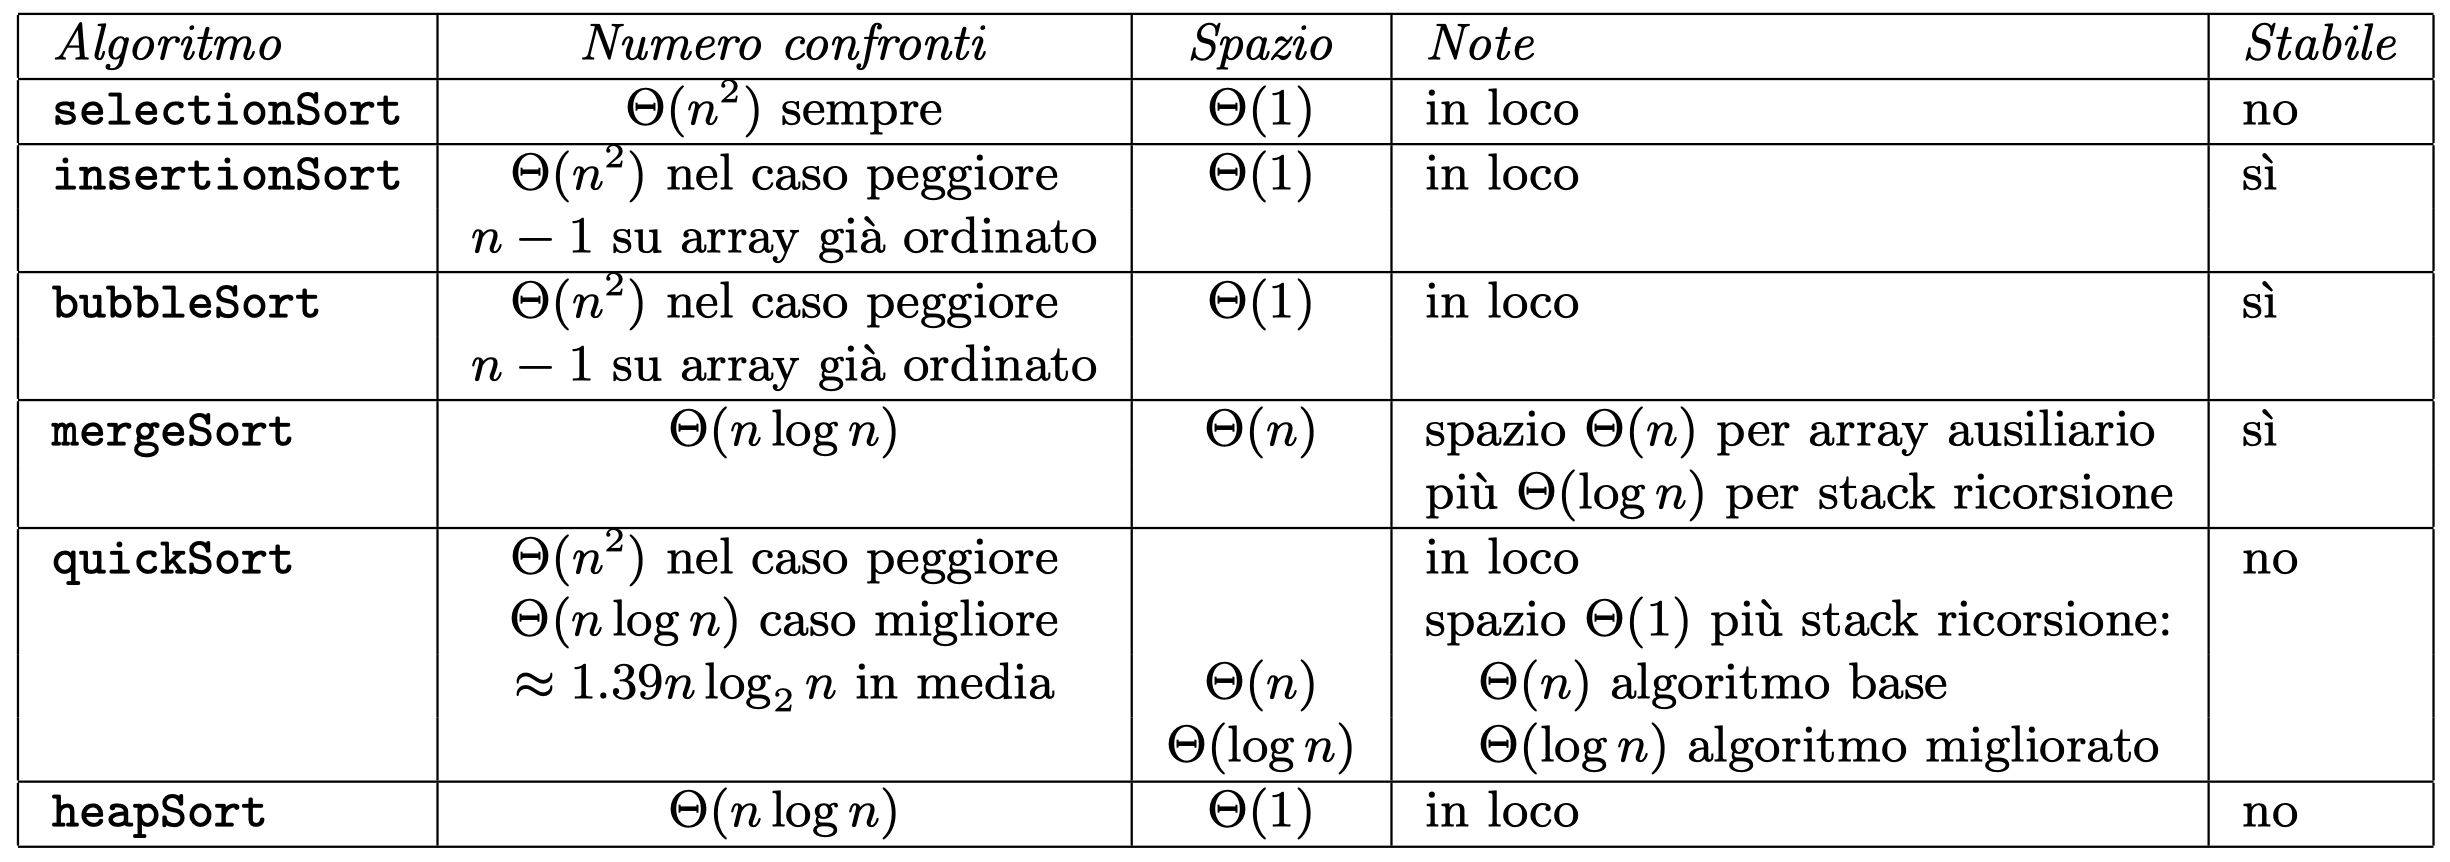
\includegraphics[width=\textwidth]{riepilogo_ordinamento.png}
\end{figure}


\subsection{Numero minimo di confronti}
Dimostreremo ora che qualsiasi algoritmo di ordinamento basato su confronti 
richiede, nel caso peggiore, un numero di confronti almeno dell'ordine di $n \log n$.
Le possibili computazioni di un algoritmo di ordinamento su sequenze di $n$ elementi 
possono essere rappresentate mediante un \emph{albero di decisione}, cioè un albero
binario in cui ciascun nodo interno rappresenta un operazione di confronto, con associati due 
sottoalberi, che dipendono dall'esito di tale operazione, mentre ogni foglia rappresenta 
una risposta dell'algoritmo, cioè un possibile ordine tra le chiavi.

\begin{center}
    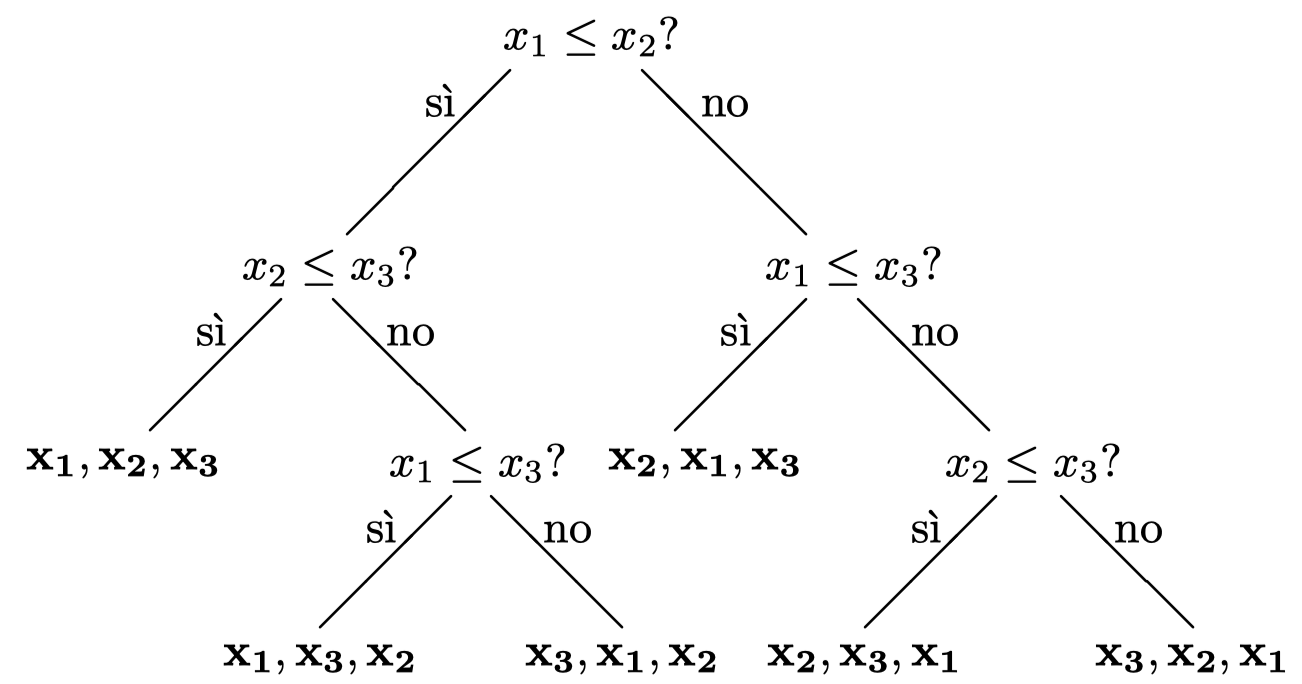
\includegraphics[scale = 0.4]{albero_decisione.png}
\end{center}
\clearpage
\noindent Indipendentemente dalla strategia utilizzata per eseguire i confronti, l'albero dovrà avere un
numero di foglie pari almeno al numero dei possibili ordini tra le chiavi, cioè
al numero di possibili permutazioni di $n$ elementi, che è $n!$. Il numero massimo
di confronti utilizzato da una strategia è pari alla profondità dell'albero.
Si può verificare che la profondità di un albero binario con $k$ foglie è
almeno logaritmica in $k$.\\
Per trovare il numero di confronti necessari nel caso peggiore stimiamo quindi 
la profondità minima che deve avere un albero con $n!$ foglie, calcolando il logaritmo di $n!$.
Utilizzando l'approssimazione di Stirling $n! \approx \sqrt{2 \pi n (\frac{n}{e})^n}$ si ottiene $\Theta(n \log n)$.\\
Possiamo concludere che \emph{ogni} algoritmo di ordinamento basato su confronti richiede nel caso peggiore 
un numero di confronti tra chiavi dell'ordine di $n \log n$ per ordinare $n$ elementi.
\clearpage
